%Chapter 2

\renewcommand{\thechapter}{2}

\chapter{Background Theory}

\section{Centroid Dynamics}


%% 4-turn formula


Closed orbit and centroid tune (which should be equivalent to bare tune, with coherent tune depression) can be reconstructed from four turns of BPM data using Koutchouk's four-turn formula [\cite{Koutchouk}]:
\begin{subequations}
\begin{equation}
\label{}
\cos \nu = \frac{x_n - x_{n+1} + x_{n+2} - x_{n+3}}{2(x_{n+1}-x_{n+2})}
\end{equation}
\begin{equation}
\label{}
x_{co} = \frac{1}{4\sin ^2 \nu/2}(x_n+x_{n+2}-2x_{n+1}\cos \nu)
\end{equation}
\end{subequations}

\section{Theory of Integrable Optics}

%% todo: clean this up (grabbed from conference paper)

\begin{figure}
\centering
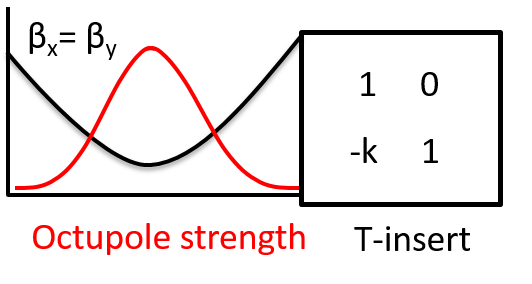
\includegraphics[width=.3\textwidth]{2.figures/toy_model.png}
\caption{Simple quasi-integrable system: FOFO focusing with nonlinear insert }
\label{fig:toymodel}
\end{figure}


Beam resonances that drive particle losses and beam halo present a significant challenge for high intensity accelerators, limiting beam current due to risk of damage and/or activation. While Landau damping can control resonant effects, the addition of weak nonlinearities to a linear lattice can introduce resonant islands and chaotic phase space orbits, which reduce dynamic aperture and lead to destructive particle loss. Theory predicts that lattices with one or two invariants and sufficiently strong nonlinear elements should suppress tune and envelope resonances without loss of stable phase space area \cite{Danilov2010}. 

The small-angle Hamiltonian for transverse particle motion in the normalized frame is given by

\begin{equation}
H_N = \frac{1}{2} \left( p_{x,N}^2 + p_{y,N}^2 +x_N^2 + y_N^2 \right) + \kappa U(x_N,y_N,s)
\end{equation}

with general nonlinear contribution $U$. (Normalized coordinates are $x_N = \frac{x}{\sqrt{\beta(s)}}$ and $p_N = p\sqrt{\beta(s)}-\frac{\alpha x}{\sqrt{\beta(s)}}$)

In order for $U$ to be an invariant quantity and for $H_N$ to be conserved, $\beta_x=\beta_y$ inside the nonlinear element and the nonlinear element strength parameter $\kappa (s)$ depends on $\beta (s)$. In particular, for an octupole element $\kappa \propto \frac{1}{\beta(s)^3}$. External focusing is provided by a linear lattice, which should reduce to an integer $\pi$ phase advance between nonlinear inserts, as depicted in Fig. \ref{fig:toymodel}. 

Parallel work at the IOTA ring \cite{antipov} will test a fully integrable nonlinear solution. The focus of the UMER nonlinear optics program is on the quasi-integrable case of the octupole lattice (with 1 invariant of motion), with the goal of experimentally observing transverse stability and halo mitigation. 